\section{Rekurentní neuronové sítě}
\label{chap:RNN}

Rekurentní neuronové sítě (ang. Recurrent Neural Networks – RNN) je kategorie
neuronových sítí, které do své architektury zapojují zpětnou vazbu. Na rozdíl
od dopředných sítí, které zpracovávají jednotlivé vstupy nezávisle, rekurentní
sítě spolu s aktuálním vstupem při evaluaci zohledňují nějakým způsobem i
výsledek předchozí iterace. Jejich využití tedy je ve dvou oblastech: analýza
změn pozorovaného objektu v čase (např. sledování pohybu, analýza chování či
predikce časových řad) a zpracování kontextuálních informací jako je např.
přirozený jazyk.

Jelikož v případě pádu se nejedná o statickou informaci, ale o jistý druh
pohybu, mohly by právě rekurentní sítě stanovit optimální cestu pro předkládané
řešení \cite{dhruv2020image}. Nyní tedy bude vysvětleno, jak rekurentní
neuronové sítě fungují a jaké jsou jejich nejpoužívanější architektury.

\subsection{Základní principy}

Data, která jsou v aktuální iteraci přebírané z předchozí iterace, se často
označují jako skrytý stav (ang. hidden state). Je to forma paměti, která se s
každou iterací aktualizuje. Často je reprezentován jako stavová vrstva (ang.
state layer nebo context layer), která přijímá hodnoty z výstupu neuronů,
uchovává je mezi iteracemi a předává je spolu se vstupními daty na vstup
neuronů. %Na obrázku \ref{fig:rnn} je tato vrstva reprezentována neurony $c_i$.

Nejjednodušší forma rekurentní neuronové sítě je NN s jednou skrytou vrstvou;
tato vrstva kromě dat ze vstupní vrstvy přijímá také výstup předchozí iterace
svých vlastních neuronů. Příklady takových sítí jsou Elmanova a Jordanova síť
\cite{elman} \cite{jordan}, které byly prvními rekurentními sítěmi
využívajícími backpropagation pro trénování.
% buď svých vlastních neuronů, anebo z neuronů výstupní vrstvy, viz obrázek
% \ref{fig:rnn}. Obrázek je zjednodušený, v praxi jsou stavová a skrytá vrstva
% plně propojeny. Tyto architektury se jmenují Elmanova síť \cite{elman}, resp.
% Jordanova síť \cite{jordan}, od jejích tvůrců. Tyto sítě jsou také známé jako
% jednoduché rekurentní sítě (ang. Simple Recurrent Networks – SRN).

% I když pojem rekurentních sítí byl známý už od začátků neuronových sítí jako
% takových a byly i případy jejích použití, právě tyto sítě patřily k prvním,
% které používaly pro trénování algoritmus backpropagation. Jednoduché rekurentní
% sítě uchovávají pouze krátkodobé vzory a jsou vhodné spíše pro jednoduché
% úlohy, jako je např. predikce časových řad.

% \begin{figure}[]
%     \centering
%     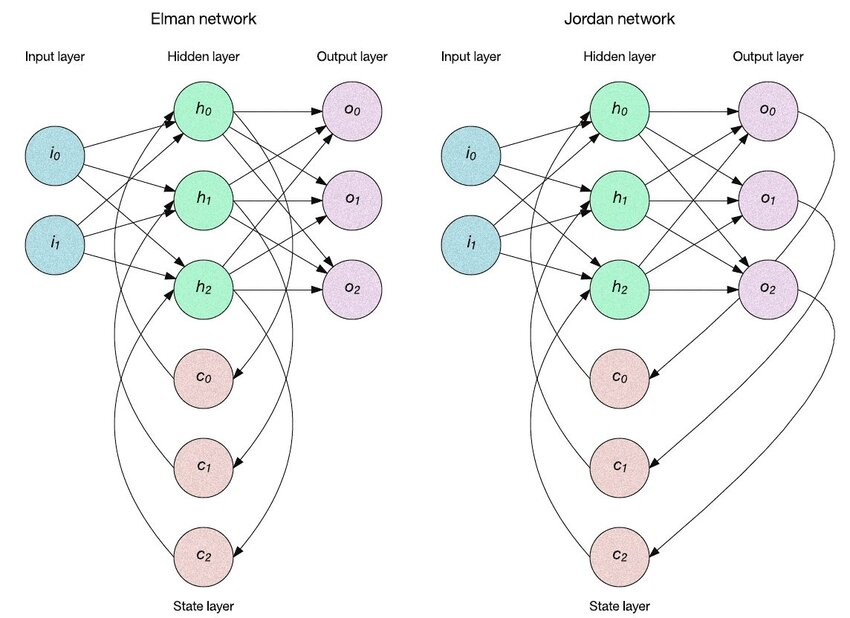
\includegraphics[width=0.8\textwidth]{Figures/rnn.png}
%     \caption{Základní architektury RNN \cite{aksoy}}
%     \label{fig:rnn}
% \end{figure}

\subsubsection*{Hluboké rekurentní sítě}

Stejně jako u dopředných neuronových sítí, kde se od jednoduchého perceptronu
přešlo k hlubokým sítím, se i rekurentní sítě rozšířily na více vrstev. V
hlubokých rekurentních neuronových sítích (ang. deep RNN – DRNN) jsou pak
jednotlivé vrstvy většinou podobné struktuře Elmanovy sítě \cite{elman} –
zpětná vazba je předávána pouze v rámci jedné vrstvy, nikoliv mezi vrstvami RNN
(například z výstupní vrstvy do první skryté vrstvy) \cite{deeprnn}. Má to
několik důvodů. Trénování sítě se zpětnou vazbou mezi vrstvami by bylo velmi
složité a obtížné. Také, u neuronových sítí obecně platí, že každá vrstva sítě
se učí pochopit problém na jiné úrovni abstrakce, zpětná vazba přes několik
vrstev by pak mohla narušit stabilitu tohoto procesu a omezit kvalitu učení.

\subsubsection*{Trénování rekurentních sítí}

Pro pochopení rekurentních neuronových sítí je třeba si vysvětlit, jak se
trénují. Pro vizualizaci trénování RNN se tyto sítě takzvaně rozbaluje v čase
(ang. unrolling). Znamená to, že jednotlivé iterace jsou vizualizovány jako
sekvence stejných sítí (stejné váhy), které v čase $t$ přijímají vstup $x_t$ a
vracejí výstup $y_t$, viz obrázek \ref{fig:bptt}. Zároveň místo smyček
znázorňujících zpětnou vazbu přijímá skrytá vrstva v čase $t$ stav $c_{t-1}$ z
předchozí iterace. Takto je propojená mezi iteracemi každá skrytá vrstva (na
obrázku \ref{fig:bptt} vizualizováno propojení přes stavovou vrstvu).

\begin{figure}[]
    \centering
    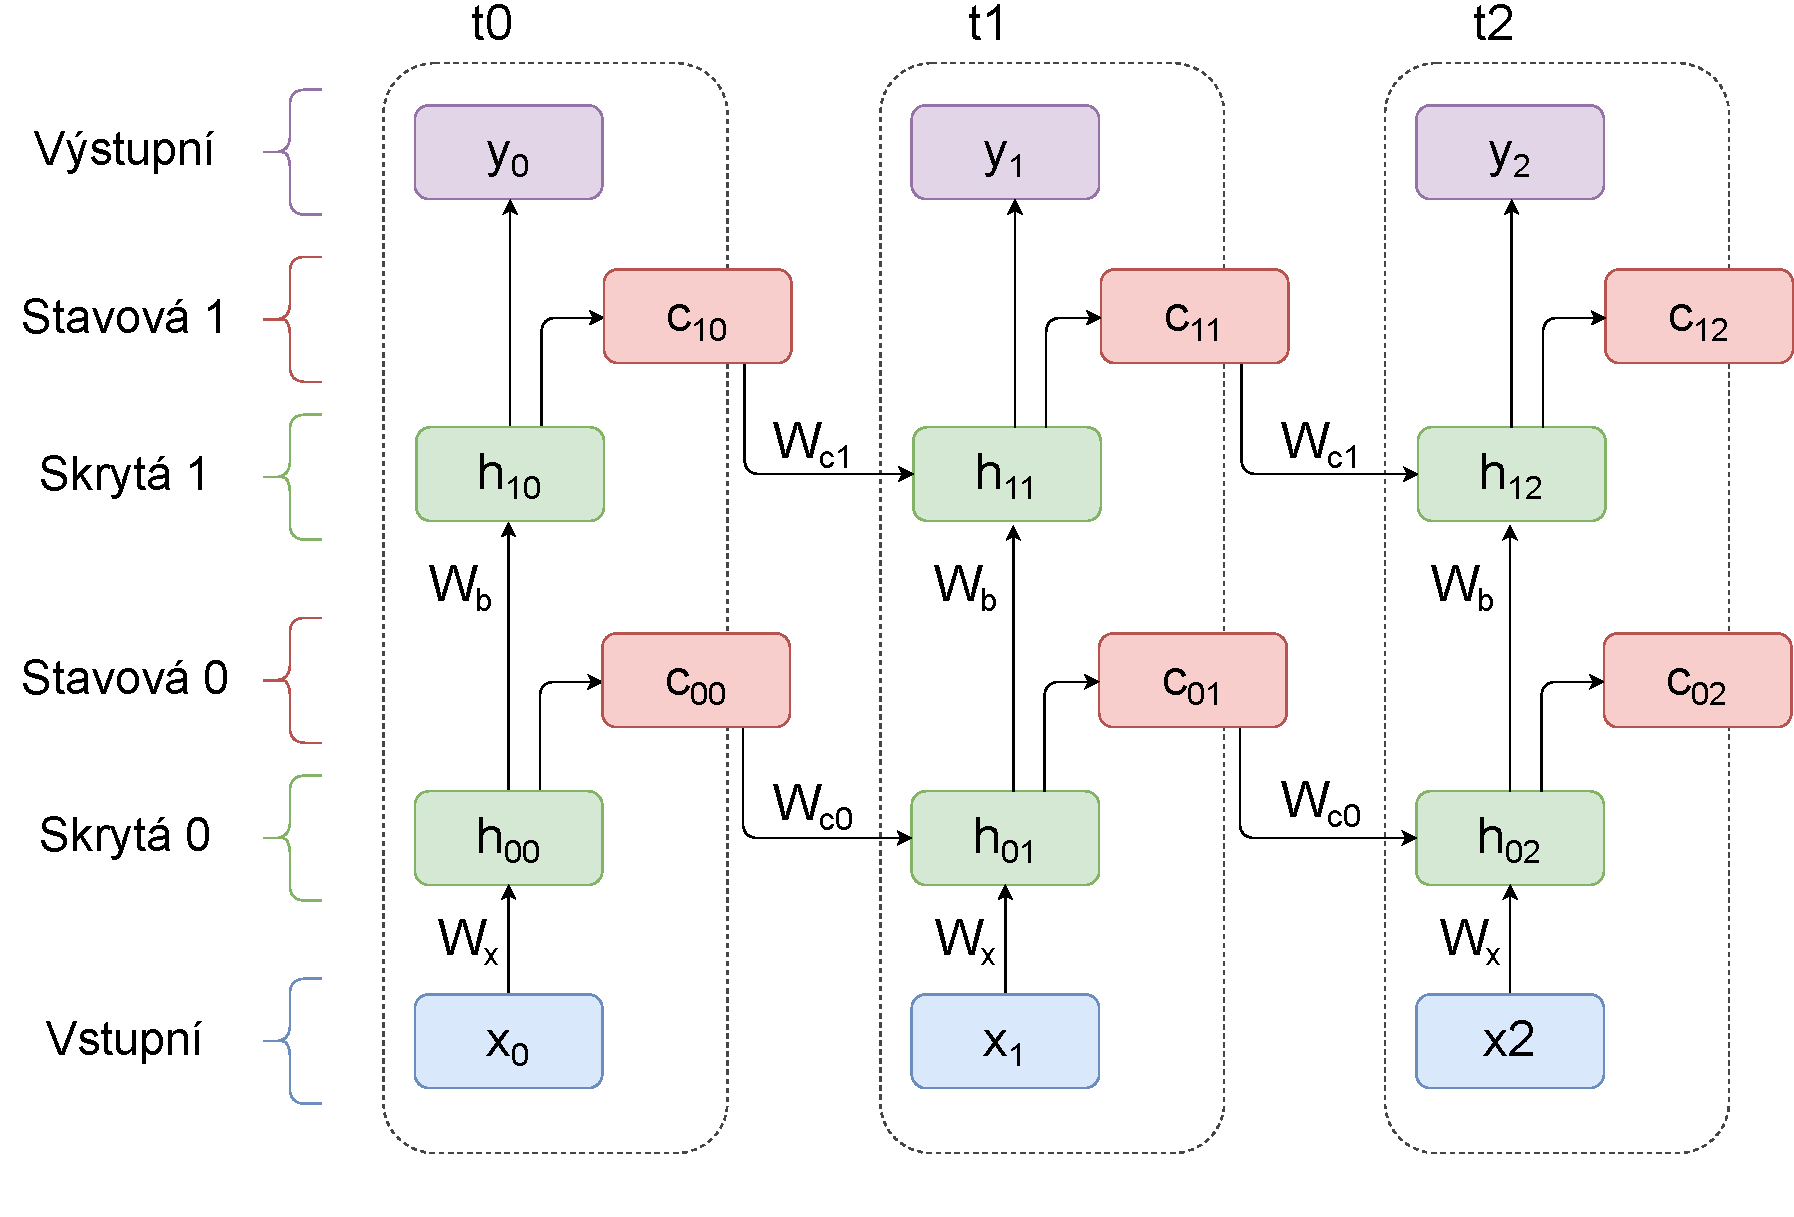
\includegraphics[width=0.75\textwidth]{Figures/BPTT.pdf}
    \caption{Unrolling hluboké RNN}
    \label{fig:bptt}
\end{figure}

Při trénování se pak používá algoritmus zpětného šíření chyby v čase (ang.
backpropagation through time – BPTT). Algoritmus funguje stejně jako klasický
backpropagation, šíří se ale nejenom vrstvami, ale i iteracemi. Unrolling
pomáhá backpropagation pochopit, jednotlivé iterace totiž jsou naskládány jako
vrstvy a celou síť řešíme jako klasickou dopřednou NN.

\subsubsection*{Problémy mizejícího a explodujícího gradientu}

Výše popsané základní rekurentní neuronové sítě, někdy označovány jako vanilla
RNN, trpí několika zásadními problémy. U dopředných sítí byl zmíněn problém
mizejícího gradientu (ang. vanishing gradient), vystupující zejména u hlubších
sítí. Ten se projevuje i u RNN a je zesílený tím, že jsou jednotlivé iterace
naskládané na sebe, podobně jako vrstvy. Zejména pak u delších sekvencí budou
mít dřívější vstupy velmi malý vliv na učení sítě.

U RNN se také projevuje problém opačný – explodující gradient (ang. exploding
gradient). Ten způsobuje, že v průběhu sekvence se váhy začnou exponenciálně
zvětšovat a dosáhnou tak nepřiměřeně velkých hodnot \cite{rnn}.

% Podívejme se, co přesně tyto problémy způsobuje. Součástí algoritmu
% backpropagation je počítání parciální derivace ztrátové funkce podle
% jednotlivých vah. V případě BPTT potřebujeme mimo jiné počítat parciální
% derivace skrytého stavu mezi jednotlivými iteracemi $\frac{\partial
%         h_{t-1}}{\partial h_t}$. Tyto derivace následně opakovaně násobíme při použití
% řetězového pravidla. Pokud je tato derivace $\frac{\partial h_{t-1}}{\partial
%         h_t}<1$, jeho vynásobení bude mít za následek postupné zmenšování gradientu.
% Pokud budeme například mít sekvencí $100$ iteraci, pak i kdyby se gradienty v
% každé iteraci zmenšovaly $0,9$ krát, po $100$ iteracích by gradient klesl na
% hodnotu $0,9^{100} \approx 2,7 \times 10^{-5}$, což je prakticky nula. Pokud se
% naopak bude gradient zvětšovat $1,1$ krát, po $100$ iteracích by gradient
% vzrostl na $1,1^{100} \approx 13 780$, což způsobí úplnou destabilizaci sítě a
% nedosáhneme žádného výsledku. Vidíme tedy, že v případě, kdy je $\frac{\partial
%         h_{t-1}}{\partial h_t}>1$, dochází k explodujícímu gradientu.

Z důvodu těchto problémů byly vyvinuty složitější rekurentní struktury. Jejich
architektura je v podstatě podobná, jednotlivé vrstvy jsou ale zastoupeny
jinými stavebními bloky, které umožňují zejména širší pochopení kontextu a
efektivnější proces trénování. Vanilla RNN se v praxi dnes využívají velmi
zřídka. K nejpoužívanějším architekturám patří LSTM (ang. long short-term
memory) a GRU (ang. gated recurrent unit), které nyní budou popsány.

\subsection{LSTM}

Dlouhá krátkodobá paměť (ang. long short-term memory – LSTM ), představena
Hochreiterem a Schmidhuberem v roce 1997 \cite{lstm}, je typ rekurentní
neuronové sítě, který byl navržen tak, aby překonal problémy mizejícího a
explodujícího gradientu.

\begin{figure}[]
    \centering
    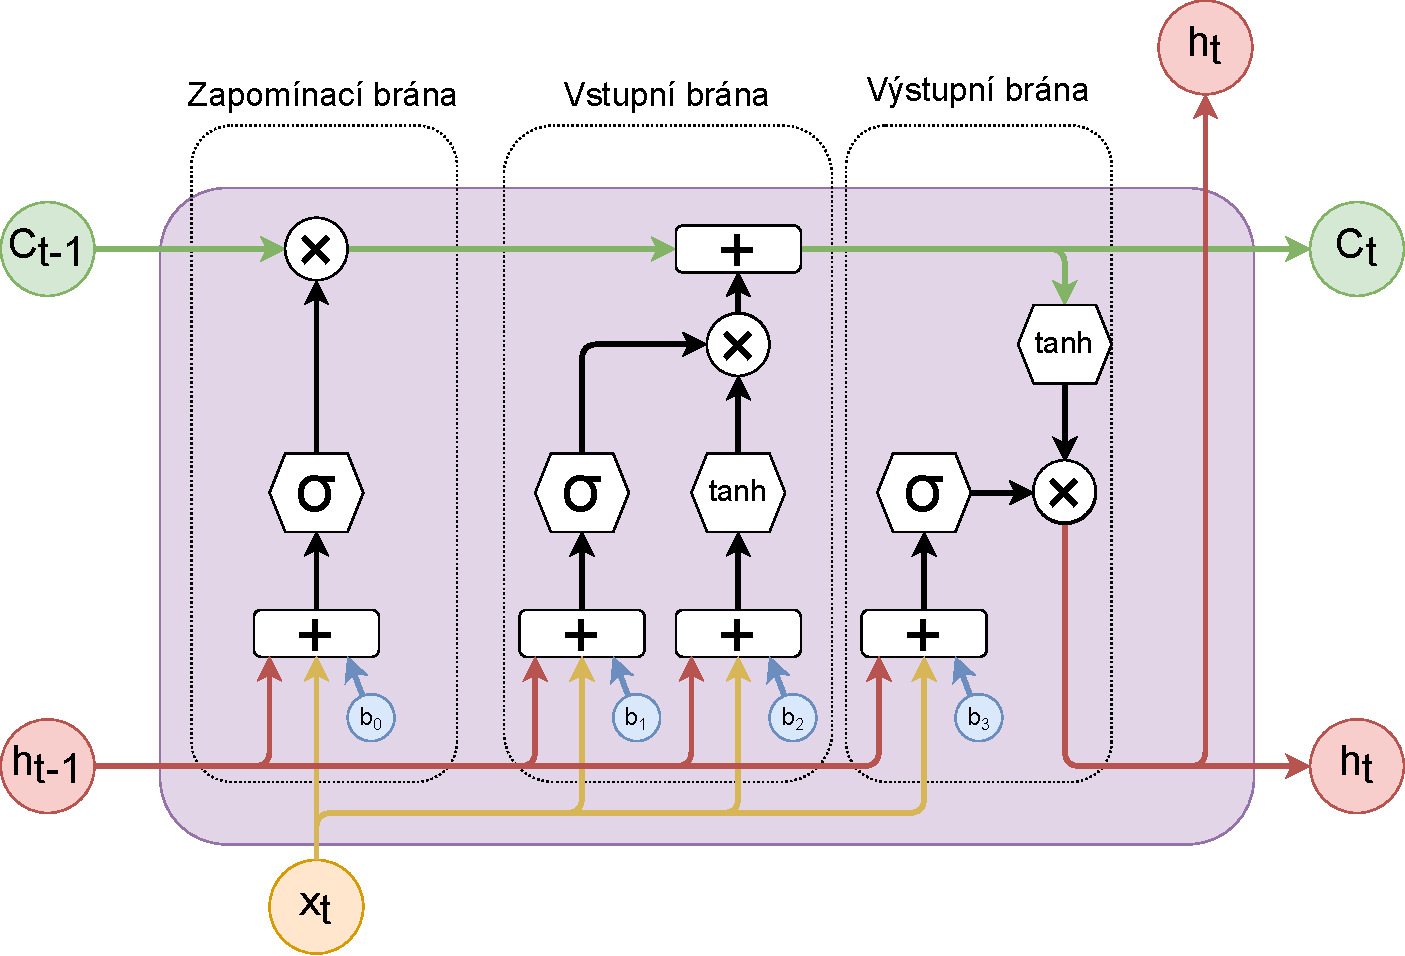
\includegraphics[width=0.7\textwidth]{Figures/LSTM_unit.pdf}
    \caption{Jednotka LSTM}
    \label{fig:lstm}
\end{figure}

Její základem je jednotka, viz obrázek \ref{fig:lstm}.1, která ve třech
stádiích aktualizuje krátkodobou a dlouhodobou paměť. Dlouhodobá paměť je
reprezentovaná pomocí stavu buňky (ang. cell state, na obrázku \ref{fig:lstm}.1
$c_t$), který je postupně upravován a nakonec předán další iteraci. Dokáže
uchovávat dlouhodobé závislosti. Krátkodobá paměť je reprezentována pomocí
skrytého stavu. Je použita pro úpravu dlouhodobé paměti, v konečném stadiu je
ale vždy v rámci dané iterace vytvořena nová. Je tak vhodná pro uchování
krátkodobých závislostí. Na obrázku \ref{fig:lstm} je znázorněna jako $h_t$.

Jednotka LSTM má tři hlavní komponenty – zapomínací bránu (ang. forget gate),
vstupní bránu (ang. input gate) a výstupní bránu (ang. output gate). Brány
určují, které informace mají být předány dál.

První, zapomínací brána určuje, které informace z dlouhodobé paměti $c_{t-1}$
se dostanou dále – co má jednotka zapomenout, resp. zapamatovat. Ve vstupní
bráně se nejprve vytvoří kandidátní stav buňky. Ten je výsledkem neuronové
vrstvy s tangenciální aktivační funkcí, do které vstupuje aktuální vstup $x_t$
a krátkodobá paměť $h_{t-1}$. Pak se určí, které informace z kandidátního stavu
buňky se přičtou do stavu buňky a vznikne tak aktuální stav buňky $c_t$. Ve
výstupní bráně se pomocí tangenciální aktivační funkce vytvoří na základě stavu
buňky $c_t$ kandidátní skrytý stav. Pak se určí, které z těchto informací budou
tvořit nový skrytý stav $h_t$.

V každé bráně tedy jsou informace, u nichž se určuje, zda je poslat dále či
nikoliv. Tyto informace zde budou označovány jako propouštěný obsah (předchozí stav buňky,
kandidátní stav buňky či kandidátní skrytý stav). Toto určení se provádí vždy
pomocí neuronové vrstvy se sigmoidní aktivační funkcí. Do těchto vrstev
vstupuje vždy předchozí skrytý stav $h_{t-1}$ a aktuální vstup $x_t$. Výstupem
je hodnota mezi $0$ a $1$ pro každou informaci. Pak se tento výsledek vynásobí
propouštěným obsahem. Pokud je výstup této vrstvy $0$, informace se nepředávají
dál, pokud je $1$, informace se předávají dále. Vstupy do všech neuronových
vrstev jsou vždy vynásobeny váhami, ty ale nejsou pro jednoduchost na obrázku
\ref{fig:lstm}.1 zobrazeny. Na obrázku \ref{fig:lstm_deep} je znázorněna
rozvinutá hluboká LSTM síť. Jednotlivé vrstvy sítě jsou naskládány vertikálně,
jednotlivé iterace pak jsou rozvinuty vedle sebe. Jednotlivé vrstvy si
předávají skrytý stav - krátkodobou paměť, mezi iteracemi si pak daná vrstva
předává krátkodobou i dlouhodobou paměť.

\begin{figure}
    \centering
    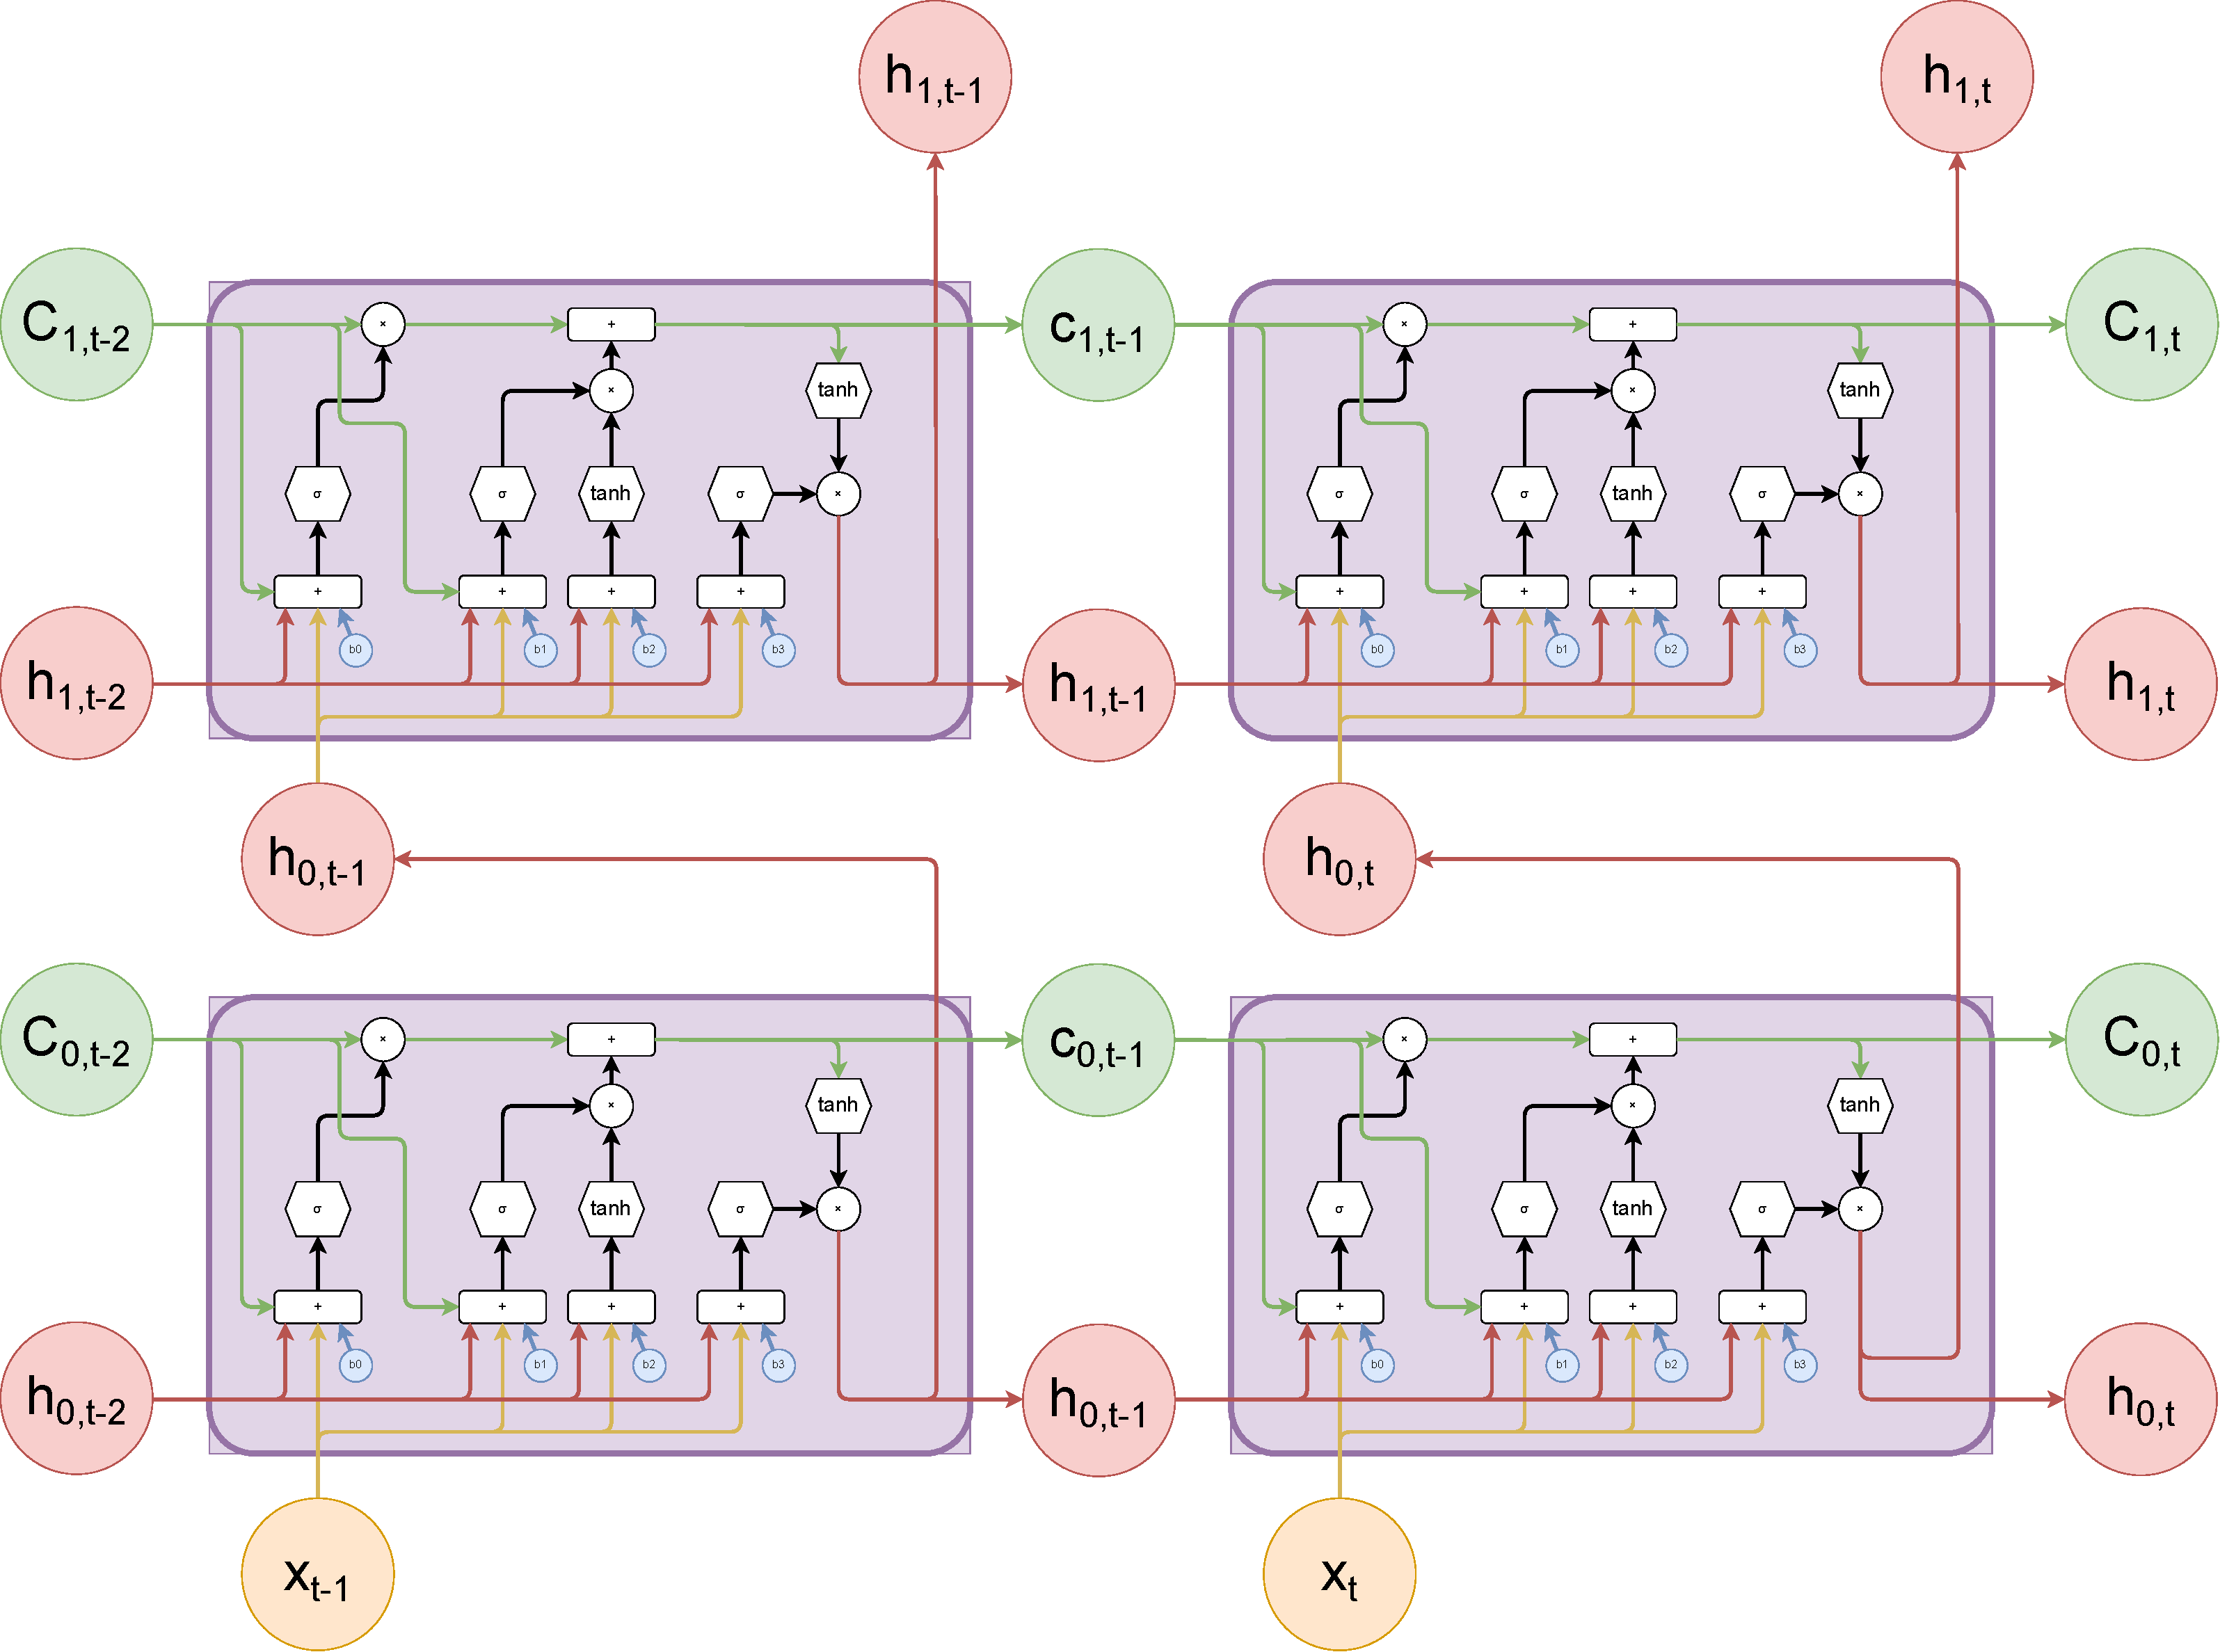
\includegraphics[width=0.70\textwidth]{Figures/LSTM_deep.pdf}
    \caption{Rozvinutá hluboká LSTM síť}
    \label{fig:lstm_deep}
\end{figure}

LSTM sítě vynikají v udržování dlouhodobých závislostí a složitých struktur.
Jelikož mají tři brány, je síť schopná přesně rozhodnout, které informace chce
dlouhodobě uchovávat, které naopak mají větší vliv na aktuální výstup a které
mají být zapomenuty. Je to ale za cenu většího výpočetního nároku a
složitějšího trénování. Také je pro tyto sítě vhodné mít větší množství
trénovacích dat, jinak může dojít k přetrénování. Využívá se tak zejména pro
predikci dlouhých a komplexních časových sekvencí či zpracování přirozeného
jazyka. Zejména u přirozeného jazyka se LSTM sítě osvědčily jako velmi
efektivní. Je totiž potřeba, aby si síť pamatovala dlouhé závislosti, zároveň
je k dispozici obrovské množství vzorků.

Síť LSTM by mohla být vhodná pro klasifikaci pózy zejména pokud by bylo potřeba
analyzovat pohyb v delších časových úsecích. Událost pádu se naopak obvykle
odehrává v krátkém čase, nicméně může se otestovat, jakých výsledků bude tato
architektura dosahovat oproti jiným rekurentním sítím, zejména v případě, kdy
modelu nebyla předávána pouze póza z $n$ posledních snímků, ale celá sekvence
detekována pro danou osobu.

\subsection{GRU}

Gated Recurrent Unit (GRU) je novější typ rekurentní neuronové sítě, který
představil v roce 2014 Cho et al. \cite{gru}. Je postavený na principu brán,
podobném jako LSTM, nepotřebuje ale zvlášť stav pro dlouhodobou paměť. Místo
toho kombinuje krátkodobou a dlouhodobou paměť do skrytého stavu $h_t$.

\begin{figure}
    \centering
    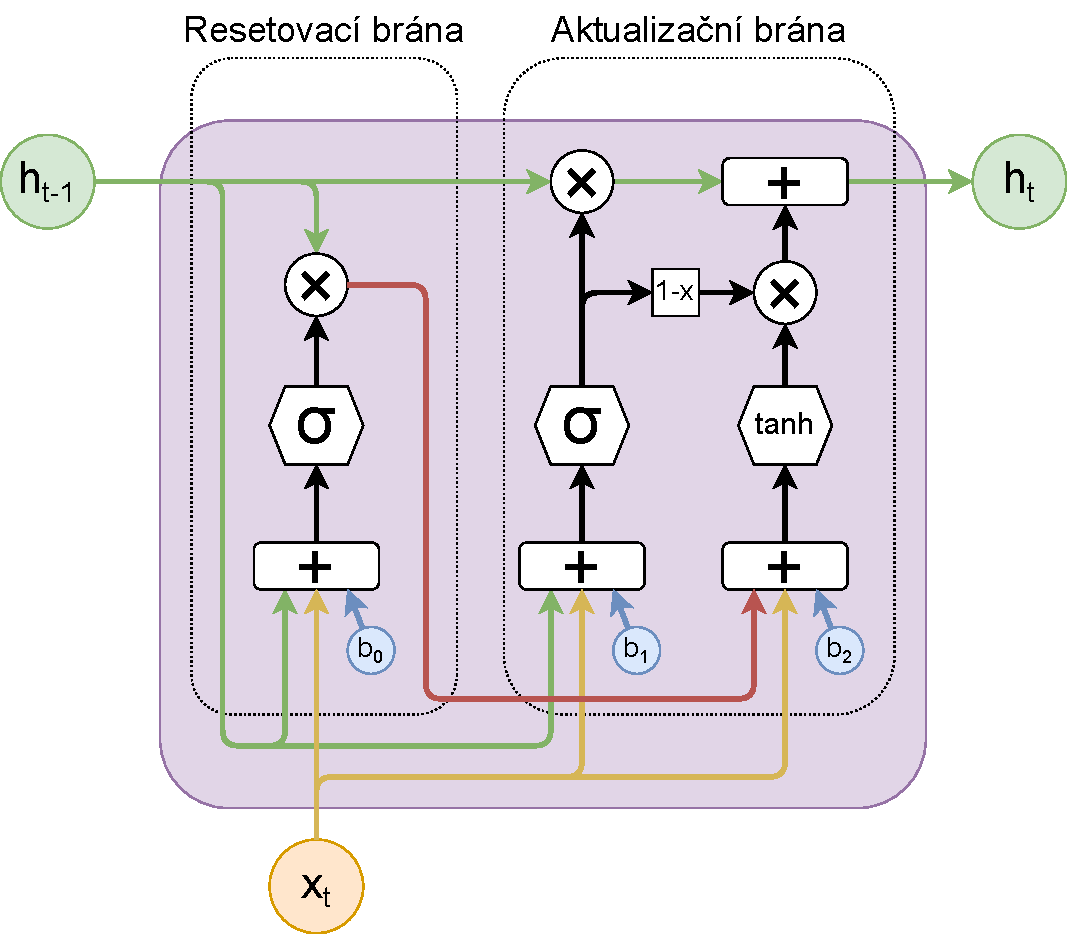
\includegraphics[width=0.6\textwidth]{Figures/GRU_unit.pdf}
    \caption{Jednotka GRU}
    \label{fig:gru_unit}
\end{figure}

GRU obsahuje dvě brány: resetovací bránu (ang. reset gate) a aktualizační bránu
(ang. update gate), viz obrázek \ref{fig:gru_unit}. V resetovací bráně se
určuje, které informace z předchozího skrytého stavu $h_{t-1}$ budou mít vliv
na tvorbu kandidátního skrytého stavu. V aktualizační bráně vzniká nový skrytý
stav $h_t$ kombinací předchozího skrytého stavu a kandidátního skrytého stavu.
Ten je vytvořen pomocí neuronové vrstvy s tangenciální aktivační funkcí, do
které vstupuje výstup resetovací brány a aktuální vstup $x_t$. Pak se na
základě předchozího skrytého stavu $h_{t-1}$ a aktuálního vstupu $x_t$ určí,
které informace v novém skrytém stavu budou převzaty z předchozího skrytého
stavu a které z kandidátního skrytého stavu.

Hlavní výhodou GRU je jednoduchost. Oproti LSTM má méně parametrů a provádí
méně výpočtů. Je tak jednak rychlejší při evaluaci, jednak jednodušší pro
natrénování. Také, u GRU sítí je menší pravděpodobnost přetrénování, což je
výhodné zejména v situacích, kdy je počet dostupných trénovacích dat omezený. GRU
sítě se často využívají v úlohách, kde je důležité rychlé zpracování a
efektivita, např. v mobilních aplikacích a zpracování v reálném čase. Je to ale
za cenu trošku horšího zpracování komplexních a dlouhodobých závislostí. Oproti
LSTM nemá GRU takovou kontrolu nad tím, které informace dlouhodobě uchovávat a
má sklon k rychlejšímu zapomínání. Proto se až tak nehodí pro složitější úlohy
a situace, kdy je nutné si pamatovat velmi dlouhé časové závislosti. Nicméně GRU sítě
jsou dneska první volbou pro mnoho úloh, po LSTM sítích se pak sahá, až když si
GRU sítě s danou úlohou neporadí.

\endinput